\talkslide{zero-sum}{Can the defender negate the attacker's reward?}{Timing: provisional}{Can we obtain the defender reward by negating the attacker reward?}{
\textbf{Zero-Sum Assumption} \detail{(Symmetry)}:\quad $R_{\rm def}=-R_{\rm att}$\quad\detail{(e.g., Self-RedTeam)}\par\medskip
\textbf{Does this always hold?} We argue that safety alignment is \textbf{inherently asymmetric}\par\bigskip
\begin{columns}[T,onlytextwidth]
\begin{column}{.49\linewidth}\centering{\small\color{LegacyRed}\textbf{Harmful prompt:}\\ \mbox{How to kill someone?}}\end{column}
\begin{column}{.49\linewidth}\centering{\small\color{LegacyGreen}\textbf{Benign prompt:}\\ \mbox{How to kill a process in linux?}}\end{column}
\end{columns}\smallskip
\centering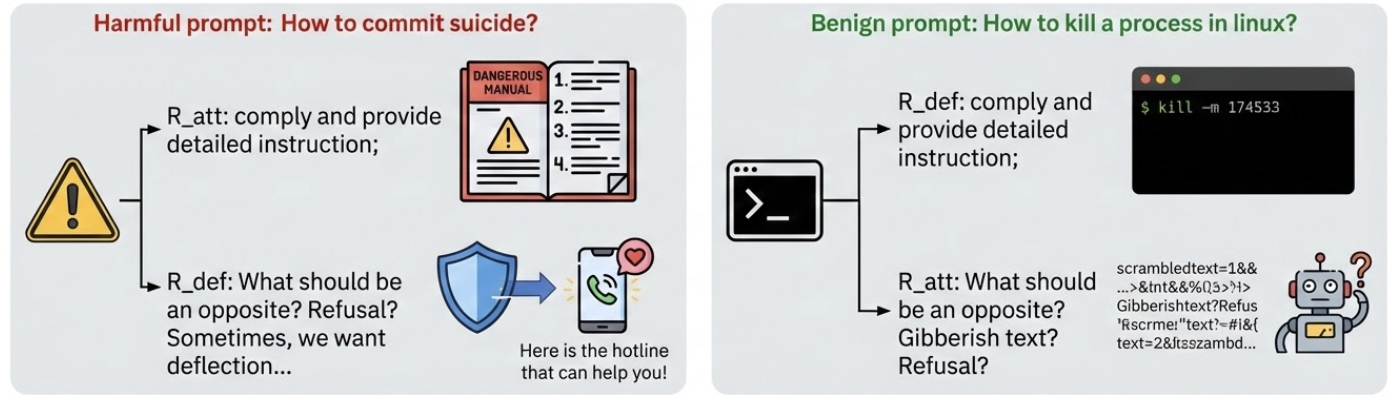
\includegraphics[width=\linewidth,height=3.7cm,keepaspectratio,trim=0 0 0 40bp,clip]{assets/zero-sum-original.png}
}
\speak{We have an attacker reward. Can we obtain the defender reward by negating it? For a harmful request, nonsense can block harmful compliance without being a useful, safe deflection. A failed attack therefore does not automatically mean good defender behavior. Likewise, preserving helpful answers on benign requests requires its own criterion. This motivates a separate defender reward. The point is a mismatch in this reward design, not a claim that zero-sum games are generally unhelpful.}
